\XtoCBlock{TrackingLoop}
\label{block:TrackingLoop}
\begin{figure}[H]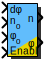
\includegraphics{TrackingLoop}\end{figure} 

\begin{XtoCtabular}{Inports}
phi\_eps & rotor angle estimation error\tabularnewline
\hline
n0 & Initial speed preloaded at rising edge of Enable signal\tabularnewline
\hline
phi0 & Initial rotor angle preloaded at rising edge of Enable signal\tabularnewline
\hline
Enable & Enable == 0: Deactivation of this block; Outputs are set to zero

Enable 0->1: Preload of angle and speed for internal integrators

Enable == 1: Activation of this block\tabularnewline
\hline
\end{XtoCtabular}


\begin{XtoCtabular}{Outports}
n & Angular speed\tabularnewline
\hline
phi & Estimated electrical rotor angle\tabularnewline
\hline
\end{XtoCtabular}

\begin{XtoCMaskParamTabular}{Mask Parameters}
\rowcolor[gray]{0.8}\textbf{Name} & \textbf{ID} & \textbf{Description}\tabularnewline\hline
Jp & 1 & Moment of inertia of rotor (and load)\tabularnewline
\hline
fo & 2 & Frequency of observer pole. The higher the pole is chosen, the more dynamic is the angle estimation\tabularnewline
\hline
p & 3 & Number of pole pairs\tabularnewline
\hline
estimation & 4 & Select where to place the emphasis of the speed output: dynamic or noise\tabularnewline
\hline
method & 5 & Discretization method of of used LTI systems (PI, I)\tabularnewline
\hline
n\_max & 6 & Maximum (mechanical) speed

(Only used for scaling in fixed point implementations)\tabularnewline
\hline
ts\_fact & 7 & Multiplication factor of base sampling time (in integer format)\tabularnewline
\hline
\end{XtoCMaskParamTabular}

\subsubsection*{Description:}
Calculates rotor angle and speed based on angle-error response due to voltage injection



BE AWARE:

For using this block with HFInjSquare-Block, set the sample time factor to 4 times the sample time factor of HFInjSquare-Block.

\subsubsection*{Implementations:}
\begin{tabular}{l l}
\textbf{FiP16} & 16 Bit Fixed Point Implementation\tabularnewline
\textbf{FiP32} & 32 Bit Fixed Point Implementation\tabularnewline
\textbf{Float32} & 32 Bit Floating Point Implementation\tabularnewline
\end{tabular}

\XtoCImplementation{FiP16}
\nopagebreak[0]

16 Bit Fixed Point Implementation

\begin{XtoCtabular}{Inports Data Type}
phi\_eps & int16\tabularnewline
\hline
n0 & int16\tabularnewline
\hline
phi0 & int16\tabularnewline
\hline
Enable & bool\tabularnewline
\hline
\end{XtoCtabular}

\begin{XtoCtabular}{Outports Data Type}
n & int16\tabularnewline
\hline
phi & int16\tabularnewline
\hline
\end{XtoCtabular}

\ifdefined \AddTestReports
\InputIfFileExists{\XcHomePath/Library/Mchp_sensorless/Doc/Test-Results/Test_TrackingLoop_FiP16.tex}{}{}
\fi
\XtoCImplementation{FiP32}
\nopagebreak[0]

32 Bit Fixed Point Implementation

\begin{XtoCtabular}{Inports Data Type}
phi\_eps & int32\tabularnewline
\hline
n0 & int32\tabularnewline
\hline
phi0 & int32\tabularnewline
\hline
Enable & bool\tabularnewline
\hline
\end{XtoCtabular}

\begin{XtoCtabular}{Outports Data Type}
n & int32\tabularnewline
\hline
phi & int32\tabularnewline
\hline
\end{XtoCtabular}

\ifdefined \AddTestReports
\InputIfFileExists{\XcHomePath/Library/Mchp_sensorless/Doc/Test-Results/Test_TrackingLoop_FiP32.tex}{}{}
\fi
\XtoCImplementation{Float32}
\nopagebreak[0]

32 Bit Floating Point Implementation

\begin{XtoCtabular}{Inports Data Type}
phi\_eps & float32\tabularnewline
\hline
n0 & float32\tabularnewline
\hline
phi0 & float32\tabularnewline
\hline
Enable & bool\tabularnewline
\hline
\end{XtoCtabular}

\begin{XtoCtabular}{Outports Data Type}
n & float32\tabularnewline
\hline
phi & float32\tabularnewline
\hline
\end{XtoCtabular}

\ifdefined \AddTestReports
\InputIfFileExists{\XcHomePath/Library/Mchp_sensorless/Doc/Test-Results/Test_TrackingLoop_Float32.tex}{}{}
\fi
